\documentclass[a4paper,10pt,notitlepage]{report}

\usepackage{datetime}
\usepackage{polski}
\usepackage[utf8]{inputenc}
\usepackage{mathtools}
\usepackage{xcolor}
\usepackage[bookmarksnumbered=white,linkbordercolor=white,citebordercolor=white]{hyperref}
\usepackage{graphicx}
\usepackage{color}
\usepackage{rotating}
\usepackage[T1]{fontenc}
\usepackage{wrapfig}
\usepackage{wallpaper}
\usepackage{float}
\usepackage[top=1cm, bottom=1.5cm, left=2cm, right=2cm]{geometry}

\makeatletter
\newcommand{\linia}{\rule{\linewidth}{0.6mm}}

\renewcommand{\maketitle}{\begin{titlepage}

    \vspace*{1cm}

    \begin{center}\small


\ThisLRCornerWallPaper{1.41}{goldenratiowallpaper}

    Środowisko programisty\\


   \huge Projekt

    \end{center}

    \vspace{3cm}

    \noindent
\linia
    \\
    \noindent
\linia
    \begin{center}

      \LARGE \textsc{\@title}

         \end{center}
\linia \\
\linia

    \vspace{0.5cm}

    \begin{flushright}

    \begin{minipage}{5cm}

    \textit{\small Autor:}\\

    \huge \textsc{\@author} \par

    \end{minipage}

     \end{flushright}

    \vspace*{\stretch{6}}

    \begin{center}

{\small Aktualna godzina i data:}
\\
    \currenttime
    \\
    \today

    \end{center}

  \end{titlepage}%
}
\makeatother

\author{\color{red}{Adam \\ Makiewicz}}

\title{\huge\ Ciąg Fibonacciego}

\linespread{1.2}
\frenchspacing

\begin{document}

\maketitle

\tableofcontents

\chapter{Historia}
\label{cha;chap1}
\section{Czym jest i jak powstał}
\label{sec;sec1.1}
{\sffamily Ciąg liczb naturalnych określony rekurencyjnie w sposób następujący:\\
    Pierwszy wyraz jest równy 0, drugi jest równy 1, każdy następny jest sumą dwóch poprzednich. Ciąg został podany w 1202 roku przez Leonarda z Pizy zwanego Fibonaccim w swoim dziele Liber abaci jako rozwiązanie zadania o rozmnażaniu się królików. Nazwę "ciąg Fibonacciego" spopularyzował w XIX w. Édouard Lucas.}\cite{wiki}
\section{Wzory}
\label{sec;sec1.2}
{\sffamily Jawny wzór na n-ty wyraz ciągu Fibonacciego podany w roku 1843 przez J.P.M. Bineta możemy otrzymać, korzystając z metody funkcji tworzących.}\cite{wiki2}
\\
\large $$ F_{n} = \frac{1}{\sqrt5}  \bigg( \frac{1+\sqrt5}{2} \bigg)^n - \frac{1}{\sqrt5}  \bigg( \frac{1-\sqrt5}{2} \bigg)^n $$
\\
Można też wyrazić wartości kolejnych elementów ciągu za pomocą symbolu Newtona :
\large $$ F_{n} = \sum_{k=1}^{\lfloor\frac{n+1}{2}\rfloor} {n-k \choose k-1} $$
\ lub za pomocą Macierzy liczb Fibonacci'ego
$$\begin{bmatrix}
       F_{n+1} \\
       F_{n}
     \end{bmatrix}=\begin{bmatrix} 1 & 1\\  1 & 0 \end{bmatrix}^n \times \begin{bmatrix} F_{1} \\  F_{0}  \end{bmatrix}$$





Oraz sumując liczby z Trójkąta Newtona:
\begin{figure}[h!]
\centering
   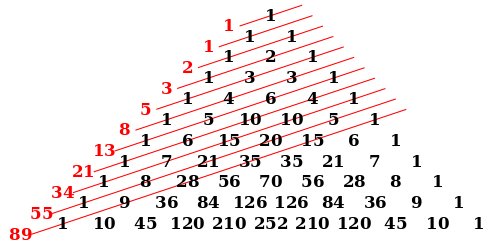
\includegraphics[scale=0.5]{LiczbyFibonacciegowTrojkaciePascala.png}
   \caption{Liczby Fibonacciego w Trojkacie Pascala}
\end{figure}
\newpage

\section{Graficzna reprezentacja Liczb Fibonacciego}
\label{sec;sec1.3}

    \begin{wrapfigure}{r}{0.5\textwidth}
  \begin{center}
    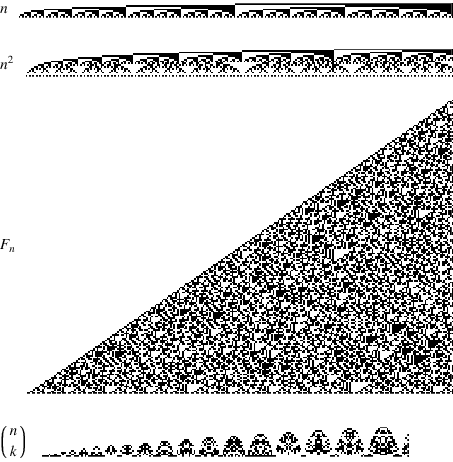
\includegraphics[width=0.5\textwidth]{BinaryPlot2.png}
  \end{center}

  \caption{Trójkąt Pascala w zapisie binarnym}
\end{wrapfigure}
 Jeśli kolejne wyrazy ciągu zapisać w systemie dwójkowym, jeden pod drugim, z wyrównaniem do prawej strony to otrzymamy wydłużający się w dół trójkąt, którego elementy powtarzają się ("czubek" pojawia się poniżej, przy prawej krawędzi, w coraz dłuższym rozwinięciu - pojawia się nad nim "biały trójkąt"), co czyni go podobnym do fraktala. W znaczeniu potocznym oznacza zwykle obiekt samo-podobny (tzn. taki, którego części są podobne do całości) albo "nieskończenie subtelny" (ukazujący subtelne detale nawet w wielokrotnym powiększeniu)Dla lepszej przejrzystości na rysunku obok wszystkie zera zastąpiono białymi punktami, a jedynki - czarnymi. \newline
 Można także przedstawić wektorowo w 3 wymiarach.
\\
 \setlength{\unitlength}{0.75mm}
\begin{picture}(60,40)
\put(30,20){\vector(1,0){30}}
\put(30,20){\vector(4,1){20}}
\put(30,20){\vector(3,1){25}}
\put(30,20){\vector(2,1){30}}
\put(30,20){\vector(1,2){10}}
\thicklines
\put(30,20){\vector(-4,1){30}}
\put(30,20){\vector(-1,4){5}}
\thinlines
\put(30,20){\vector(-1,-1){5}}
\put(30,20){\vector(-1,-4){5}}
\end{picture}
\\\\\\
\sffamily \colorbox{yellow}{Złota liczba}
\\
\ttfamily{\color{white}Granica ciągu czyli ilorazów sąsiadujących ze sobą wyrazów ciągu Fibonacci'ego \\to tzw. złota liczba lub złota proporcja definiowana jako dodatnie rozwiązanie\\ równania
$$\lim_{n \to \infty} {\frac{F(n+1)}{F(n)} =\phi}$$
\\
$$\varphi=\frac{1+\sqrt5}{2}\approx 1.6180339887...$$
\\\\\\\\\\\\\\\\\\
\
\
\
gdzie liczba $\varphi$ tworzy spiralę logarytmiczną

}
\ThisLRCornerWallPaper{1.0}{golden}




\chapter{\color{green}Przykłady Liczb Fibonacciego w naturze}
\label{cha;chap2}
\section{\color{orange}Ludzkie proporcje}


\begin{flushleft}
\includegraphics[scale=1]{figure}\
\end{flushleft}
Stosunek długości kości:
\begin{tabular}[H]{|| l || c || r ||}
			\hline
			\hline
			1 & 1 & 2 \\ \hline
			3 & 5 & 8 \\ \hline
			13 & 21 & 34 \\
			\hline
			\hline
  \end{tabular}
\\
Niektórzy doszukują się złotej proporcji wszędzie...\\
\begin{flushright}
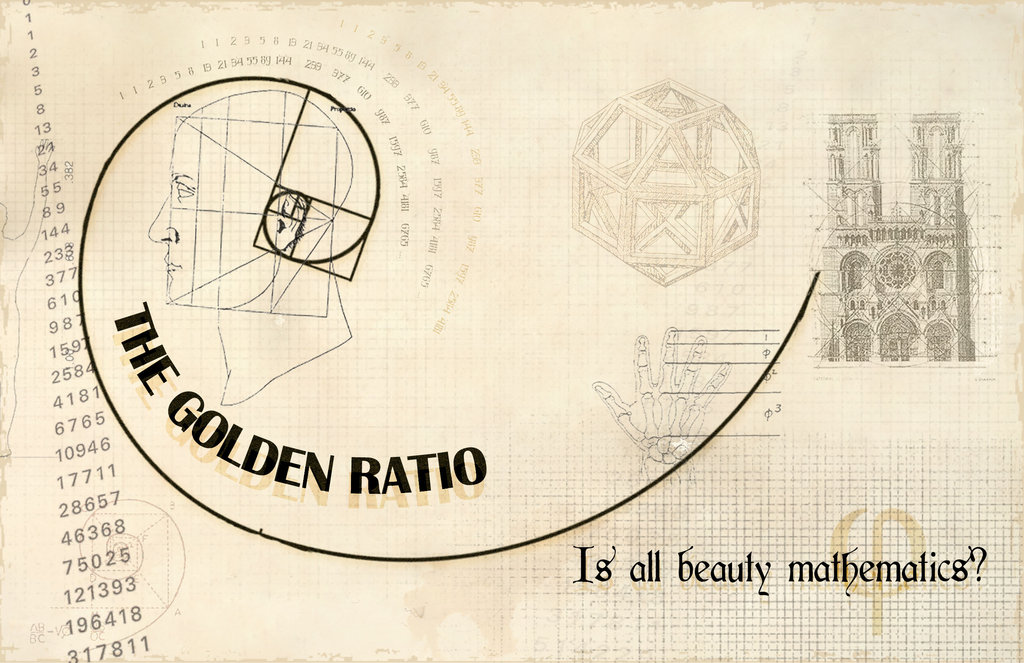
\includegraphics[width=\textwidth, angle=70, scale=0.5]{thegoldenratio} 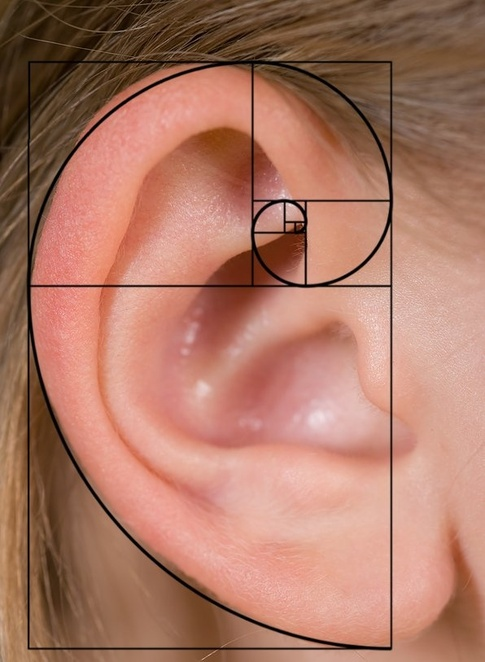
\includegraphics[scale=0.3, angle=45]{naturespiral}
\end{flushright}

\section{\color{blue}Przykłady z natury}
\label{sec;sec2.2}
\begin{flushleft}
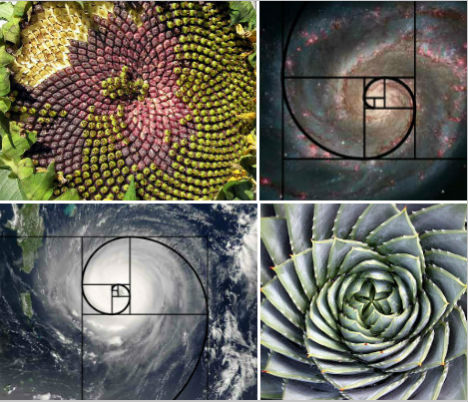
\includegraphics[width=\textwidth]{golden-spiral-main} 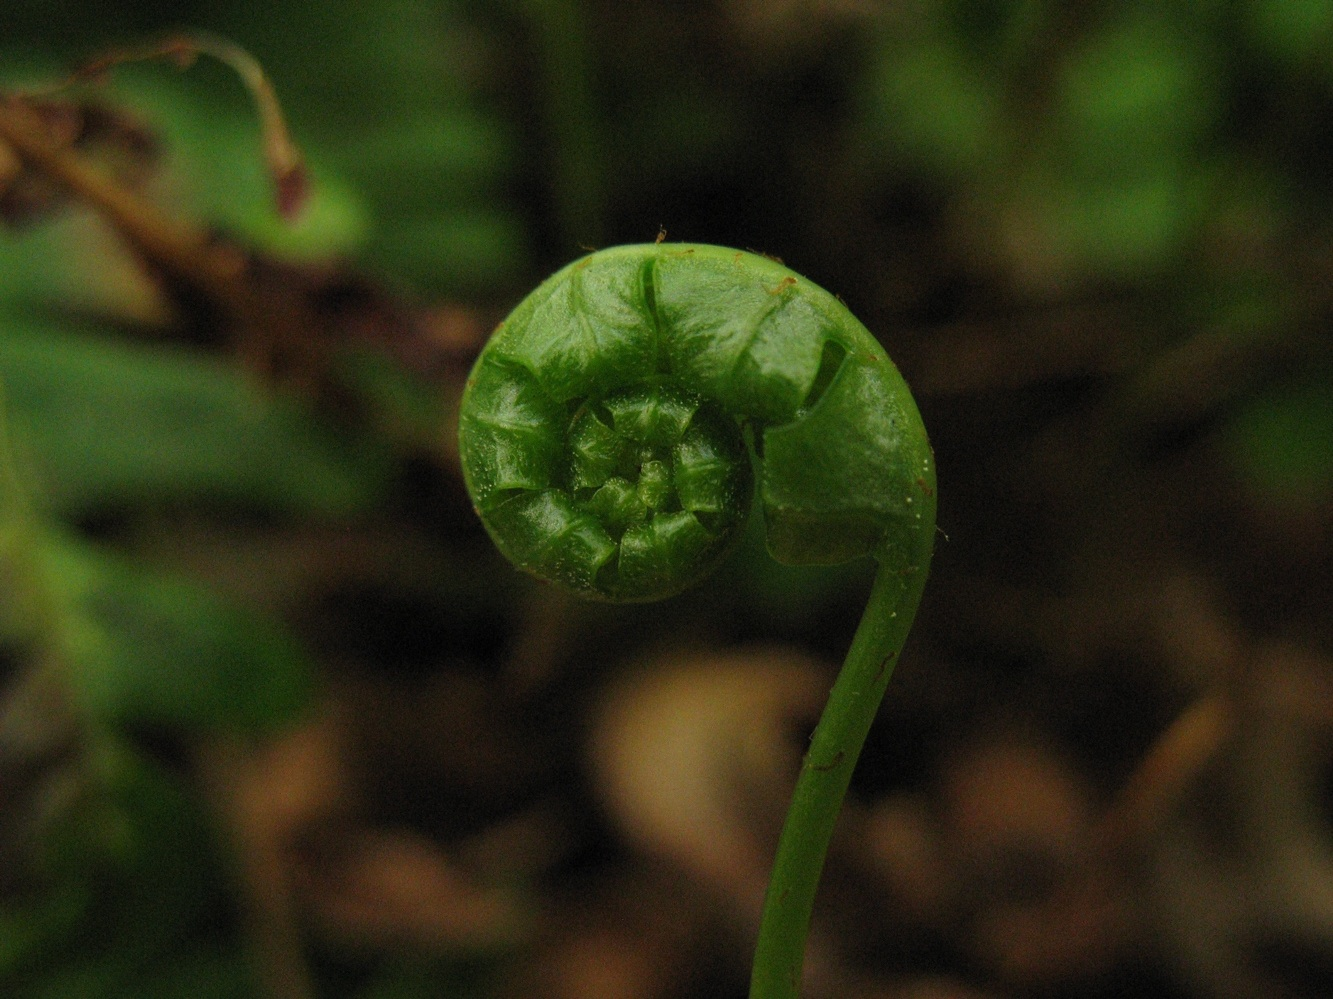
\includegraphics[width=192pt, height=252pt]{fib1}
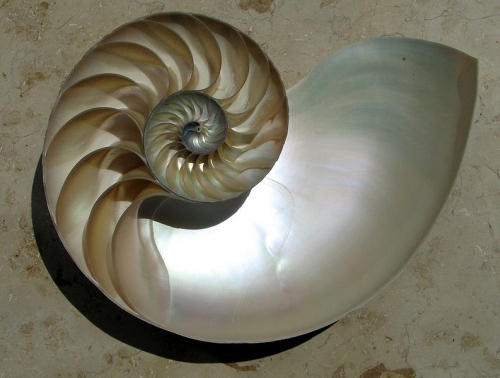
\includegraphics[width=10cm, height=9cm]{nautilussection}
\end{flushleft}




\newpage
\section{Fraktale}
\label{sec;sec3.3}
{\upshape Fraktal (łac. fractus – złamany, cząstkowy, ułamkowy) w znaczeniu potocznym oznacza zwykle obiekt samo-podobny (tzn. taki, którego części są podobne do całości) albo "nieskończenie subtelny" (ukazujący subtelne detale nawet w wielokrotnym powiększeniu). Ze względu na olbrzymią różnorodność przykładów matematycy obecnie unikają podawania ścisłej definicji i proponują określać fraktal jako zbiór, który posiada wszystkie poniższe charakterystyki albo przynajmniej ich większość:\cite{wiki3}}
\begin{itemize}
  \item
\begin{description}
  \item[First] \hfill \\
 \colorbox{orange}{ ma nietrywialną strukturę w każdej skali, }
  \item[Second] \hfill \\
 \colorbox{yellow}{ struktura ta nie daje się łatwo opisać w języku tradycyjnej geometrii euklidesowej, }
  \item[Third] \hfill \\
 \colorbox{black}{{\color{white}jest samo-podobny, jeśli nie w sensie dokładnym, to przybliżonym lub stochastycznym,\ldots}}
\end{description}
\end{itemize}

\chapter{Obrazki}
{\rmfamily .}
\label{cha;chap4}
\section{Matematyczne}
\label{sec;sec4.1}



\begin{center}
\setlength{\unitlength}{5cm}
\begin{picture}(1,1)
\put(0,0){\line(0,1){1}}
\put(0,0){\line(1,0){1}}
\put(0,0){\line(1,1){1}}
\put(0,0){\line(1,2){.5}}
\put(0,0){\line(1,3){.3333}}
\put(0,0){\line(1,4){.25}}
\put(0,0){\line(1,5){.2}}
\put(0,0){\line(1,6){.1667}}
\put(0,0){\line(2,1){1}}
\put(0,0){\line(2,3){.6667}}
\put(0,0){\line(2,5){.4}}
\put(0,0){\line(3,1){1}}
\put(0,0){\line(3,2){1}}
\put(0,0){\line(3,4){.75}}
\put(0,0){\line(3,5){.6}}
\put(0,0){\line(4,1){1}}
\put(0,0){\line(4,3){1}}
\put(0,0){\line(4,5){.8}}
\put(0,0){\line(5,1){1}}
\put(0,0){\line(5,2){1}}
\put(0,0){\line(5,3){1}}
\put(0,0){\line(5,4){1}}
\put(0,0){\line(5,6){.8333}}
\put(0,0){\line(6,1){1}}
\put(0,0){\line(6,5){1}}
\end{picture}
\end{center}

\section{Kurczak}
\label{sec;sec4.2}
\begin{center}
\begin{turn}{30}
\includegraphics{kurczak.png}
\end{turn}
\includegraphics[scale=0.5, angle=180]{kurczak.png}
\includegraphics[width=2.5cm]{kurczak.png}
\includegraphics{kurczak.png}
\end{center}
\begin{figure}[h!]
  \caption{Oto kurczak}
  \centering
    \includegraphics[width=0.5\textwidth]{kurczak.png}
\end{figure}


\begin{thebibliography}{1}

\bibitem{wiki}\url{http://pl.wikipedia.org/wiki/Ci%C4%85g_Fibonacciego}
\bibitem{wiki2}\url{http://pl.wikipedia.org/wiki/Wz%C3%B3r_Bineta}
\bibitem{wiki3}\url{http://pl.wikipedia.org/wiki/Fraktal}

\end{thebibliography}



\end{document}

